%!TEX root = ../../template.tex
%%%%%%%%%%%%%%%%%%%%%%%%%%%%%%%%%%%%%%%%%%%%%%%%%%%%%%%%%%%%%%%%%%%%
%% data_flow_and_interaction.tex
%% Data Flow and Interaction section for Proposed Model and Implementation
%%%%%%%%%%%%%%%%%%%%%%%%%%%%%%%%%%%%%%%%%%%%%%%%%%%%%%%%%%%%%%%%%%%%

\section{Data Flow and Interaction}
\label{sec:ProposedModelDataFlowAndInteraction}

This section describes the main data flows happening in the platform, showing how components interact and why each flow is structured the way it is. Each subsection covers a different flow: ingestion, analytics, and historical queries. The specific topic names, endpoints, and configuration values for these flows can be found in Table~\ref{tab:kafka-topics} and Chapter~\ref{cha:Implementation}.

\subsection{Telemetry Ingestion Flow}
This flow covers the path a telemetry message takes from a physical device all the way to the database. It starts when a device publishes a \gls{JSON} payload to the \gls{MQTT} broker on its device-specific topic. The broker has already authenticated the device during the connection handshake, so it accepts the message under \gls{QoS} level 1 and sends an acknowledgment back. The \gls{MQTT}-Kafka bridge then picks up the message and forwards it to the raw telemetry topic on Kafka (see Table~\ref{tab:kafka-topics}). The main cloud ingestion path is shown in Figure~\ref{fig:telemetry-ingestion-flow}.

The Ingestion Service consumes this message, flattens the \gls{JSON} payload into individual key-value pairs, and publishes each data point as a separate normalized event on \texttt{telemetry.events}. From that point, the stream fans out to independent consumers. The Storage Service writes the normalized data to TimescaleDB for historical queries, the Metadata Service registers previously unseen device-key pairs, the Analytics Service evaluates rules and anomaly detectors, and the Read Service forwards live updates to connected clients. This separation keeps the publishing path independent from database writes and metadata updates. If one downstream consumer slows down or fails, the others can continue processing the same stream.

\gls{QoS} level 1 gives at-least-once delivery between the device and the \gls{MQTT} broker: the device retransmits if it does not get an acknowledgment. Once the bridge sends the message to Kafka, Kafka's durable log makes sure no message is lost even if a consumer crashes or restarts. Put together, these two guarantees mean that once the broker accepts a telemetry message, it will eventually reach the database regardless of failures along the way.

Once normalized, the events are ready for downstream processing. The Analytics Service picks them up to check against monitoring rules, and the Read Service picks them up to push real-time updates to the web application. Both of these flows are described below.

For devices that use \gls{HTTP} or \gls{CoAP} instead, the Protocol Adapter authenticates the device and publishes the payload to the same raw telemetry topic that the \gls{MQTT}-Kafka bridge uses. From that point on, the data goes through the exact same pipeline.

The Protocol Adapter also handles binary file uploads from devices. When a device sends a file over \gls{HTTP}, the adapter stores it in MinIO and emits a metadata event to the \texttt{file.uploads} Kafka topic containing the object key, content type, file size, and a download \gls{URL}. This path is separate from the telemetry pipeline: files go to object storage instead of TimescaleDB, and the metadata event carries a reference to the stored object rather than the data itself. No service currently consumes this topic, but the event is available for future capabilities such as image analysis or automated processing, following the same extensibility model that the rest of the Kafka architecture provides.

Telemetry from the edge follows the write-first pattern described in Section~\ref{sec:EdgeNode}. Once the data reaches the cloud broker, the bridge routes it to a dedicated Kafka topic for pre-normalized data. The Ingestion Service consumes that topic, skips the flattening step, and republishes the payload to \texttt{telemetry.events}. From there, the edge data follows the same cloud path as any other normalized telemetry: the Storage Service persists it, the Metadata Service updates the known key set, the Analytics Service evaluates it when appropriate, and the Read Service can deliver it in real time. This edge-specific path is shown in Figure~\ref{fig:edge-telemetry-flow}.

\begin{figure}[htbp]
    \centering
    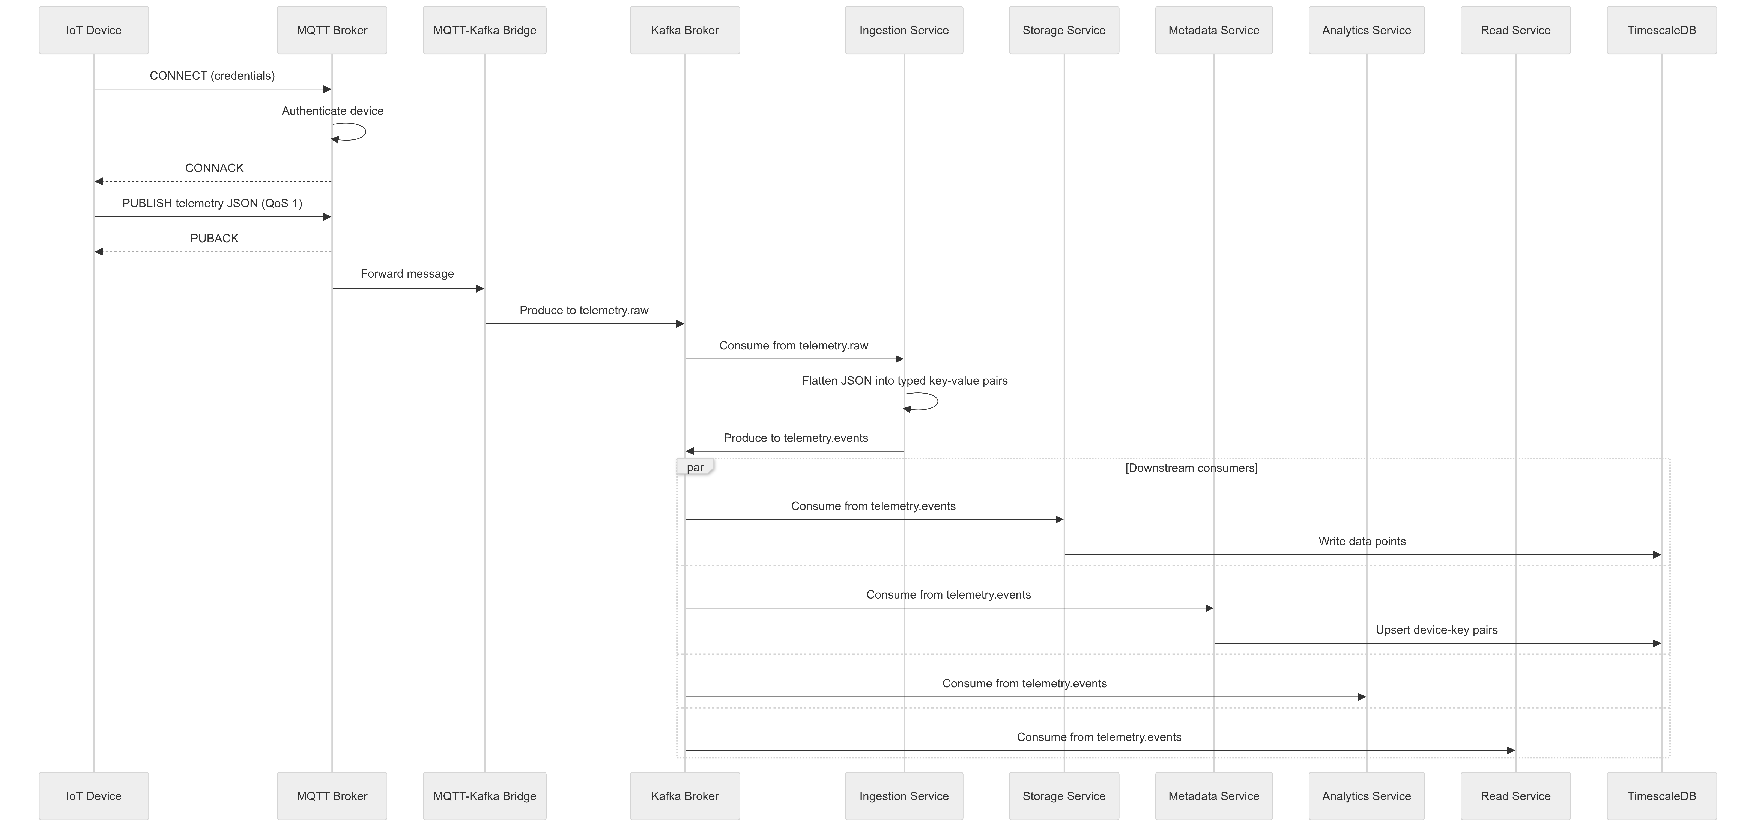
\includegraphics[width=\textwidth]{Chapters/Figures/DataFlow/TelemetryIngestionFlow.pdf}
    \caption{Telemetry ingestion sequence diagram.}
    \label{fig:telemetry-ingestion-flow}
\end{figure}

\begin{figure}[htbp]
    \centering
    \includegraphics[height=0.95\textheight]{Chapters/Figures/DataFlow/EdgeTelemetryIngestionFlow.pdf}
    \caption{Edge telemetry ingestion flow, showing local write-first persistence, periodic retry during connectivity loss, and reintegration into the cloud processing pipeline.}
    \label{fig:edge-telemetry-flow}
\end{figure}

\subsection{Analytics and Alert Flow}
This flow starts where ingestion ends: with normalized telemetry events sitting on Kafka. The Analytics Service consumes each event and checks it against the monitoring rules that apply to that device. If a rule fires, the service checks for duplicates so the same alert is not emitted multiple times, then publishes an alert event to the standard alert stream. The event carries the snapshot information needed to understand the alert later: the rule context, the threshold values, the triggering value, the device, and the user that should be notified. The Storage Service consumes that event and stores it in TimescaleDB. This keeps detection and persistence decoupled while preserving the full alert context. If the Kafka emission fails, the event goes to a dead-letter topic for periodic retry, following the same recovery pattern used in the telemetry pipeline. The main alert path is shown in Figure~\ref{fig:analytics-alert-flow}.

The Analytics Service also runs statistical anomaly detection on every numeric event. Anomaly alerts use the same path as rule-based alerts: analytics emits them to \texttt{alerts.events}, storage persists them, and the downstream delivery services consume the same event stream.

From there, the Read Service pushes each alert over WebSocket to the target user's connections, and the Notifications Service sends email notifications based on the user's preferences and severity filters.

Alerts from the edge take a different route but end up in the same place. The edge node checks telemetry against its locally cached highest-severity rules (Section~\ref{subsec:LocalAnalyticsImpl}), applies deduplication, and stores any alerts it generates. If the cloud connection is available, the alerts are sent directly to the cloud broker. Otherwise, they wait for the next sync cycle (Section~\ref{subsec:DataSyncImpl}). Once an edge alert reaches the cloud, the Analytics Service forwards it to the standard \texttt{alerts.events} stream. The Storage Service then persists it using the same alert model used for cloud-generated alerts. From that point on, there is no difference between an edge alert and a cloud alert: it is sent over WebSocket, appears in the alert history, and triggers emails in the same way. This edge path is also included in Figure~\ref{fig:analytics-alert-flow}.

\begin{figure}[htbp]
    \centering
    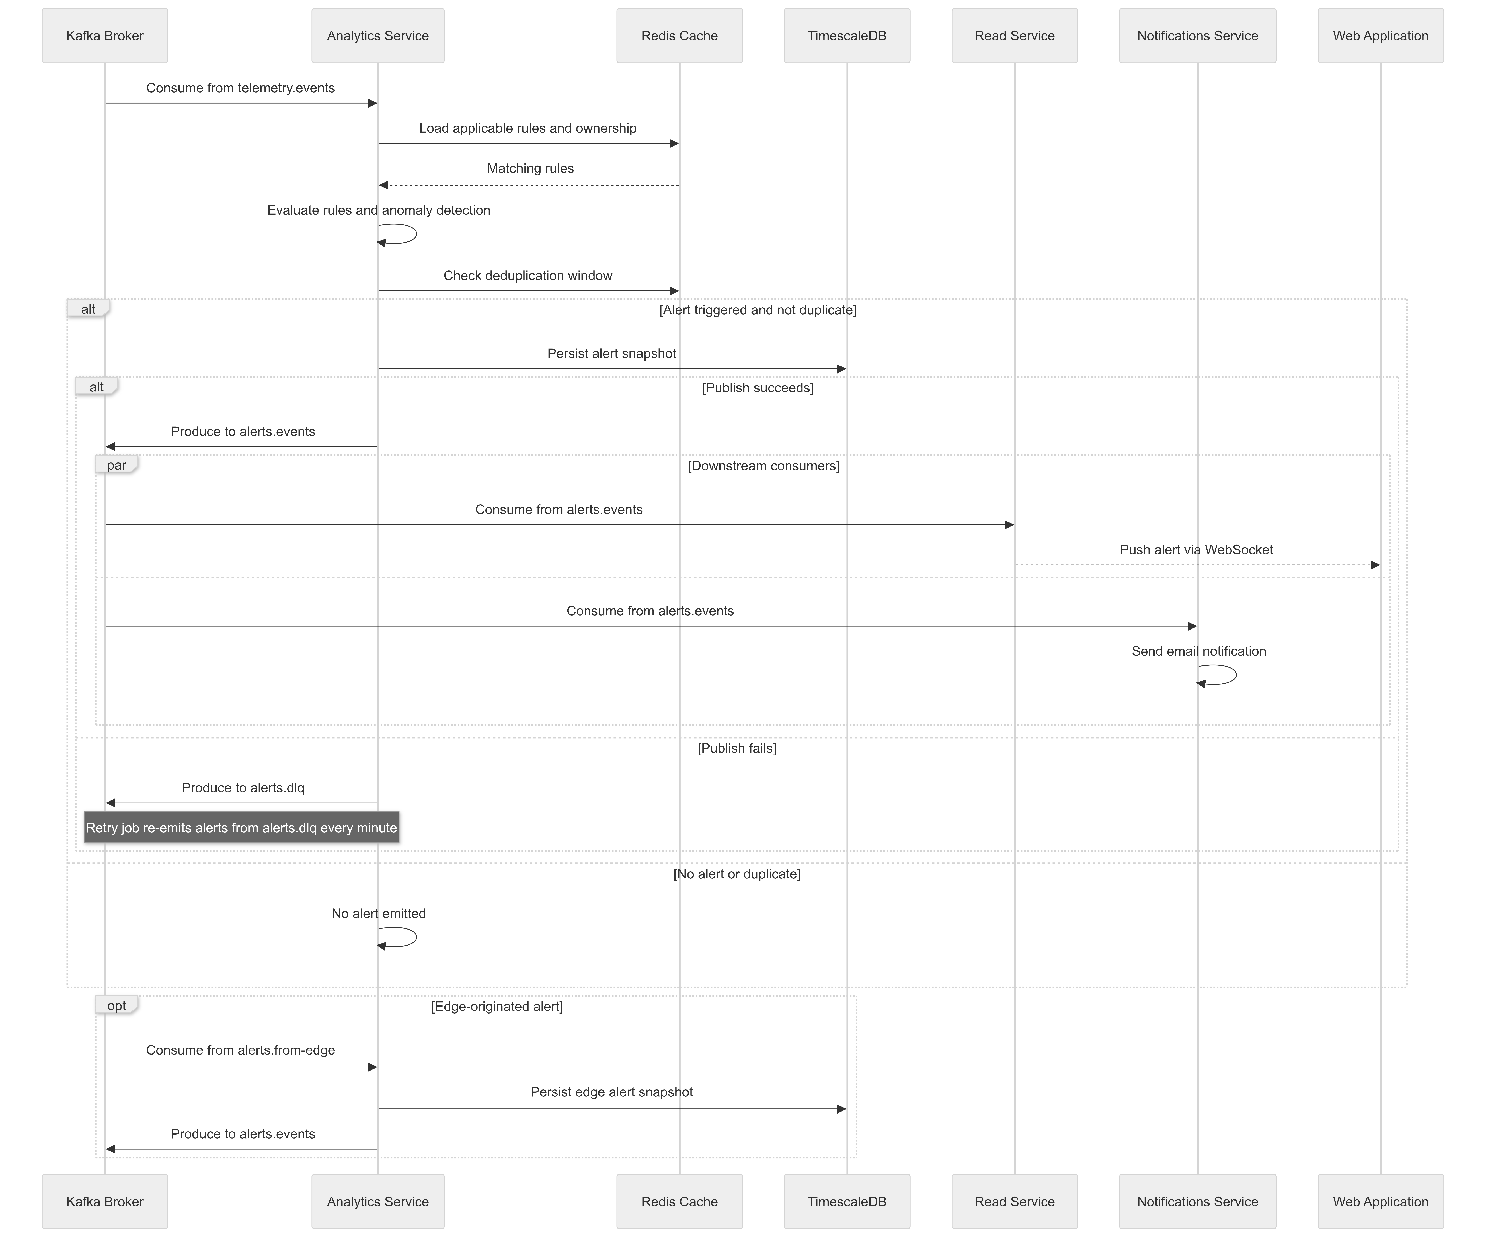
\includegraphics[width=\textwidth]{Chapters/Figures/DataFlow/AnalyticsAlertsFlow.pdf}
    \caption{Analytics and alert flow, showing rule evaluation, deduplication, alert persistence, event emission, and downstream delivery to WebSocket and email consumers.}
    \label{fig:analytics-alert-flow}
\end{figure}

\subsection{Historical Data Query Flow}
The flows above cover the write path: data arriving from devices, getting processed, and generating alerts. This flow covers the read path, where the web application fetches stored data for dashboards and analysis. Unlike the write path, which is event-driven, the read path is synchronous and follows a standard request-response pattern through the \gls{API} Gateway.

When the web application needs historical telemetry, it sends an \gls{HTTP} request to the \gls{API} Gateway. The gateway authenticates the request and forwards it to the Read Service, which queries TimescaleDB with the appropriate time range. Alert queries work the same way: the web application asks the Read Service through the gateway, filtering by device, acknowledgment status, or date range.

Alert acknowledgment is the exception. Since it is a write operation, the gateway routes it to the Analytics Service instead of the Read Service.
